\section*{Assignment 05: Governance and Data Policies}
\addcontentsline{toc}{section}{Assignment 05: Governance and Data Policies}

\subsection*{Onboarding, feedback loops, and moderation}
SkillSync onboarding mixes storytelling and friction-testing. Students and NGOs see separate landing flows that foreground portfolio wins or social-impact outcomes before everyone enters a guided tour of the core interactions. The sequence stays lean:
\begin{itemize}
  \item pre-signup nudges that point to sample projects and set expectations,
  \item profile setup with defaults for skills, availability, and preferences,
  \item a ``first mission'' checklist unlocking badges only after critical actions.
\end{itemize}

Feedback loops sit inside the flow: after each core action we collect a one-click rating plus optional note, slice results in cohort dashboards, and follow up when a group slips. Weekly summaries keep both sides accountable so we can tweak rules while the experience still feels fair \citep{Reillier2017}. Moderation runs on three layers: automated filters for obvious risks, community stewards who can hide content temporarily, and a professional response team that closes escalations within 24 hours.

\subsection*{Data policies and ethics}
Data collection sticks to a minimality principle: we capture only what matching and trust require (profile basics, transaction history, quality feedback) because over-collection erodes legitimacy \citep{Zuboff2019}. Service improvement comes first, then responsible personalisation, and only then aggregated insights; differential privacy, export audits, and fairness checks catch edge cases \citep{Srnicek2017}.

Transparency matters, so we ship a ``data mirror'' where students and organisations can inspect every datapoint we hold, tweak retention choices, and delete items when needed, then publish quarterly accountability notes with moderation stats, security incidents, and algorithm updates while an internal ethics review board forces product teams to justify experiments so power does not drift \citep{Choudary2016,Lecture10}.

Figure~\ref{fig:onboarding-flow} shows the four-step carousel that keeps the welcome checklist on top so the first mission completes in under fifteen minutes; guided tasks unlock contextual tips and short videos, and completion of the first three steps jumped from 54\% to 83\% (n=58).

\begin{figure}[H]
  \centering
  \makebox[\textwidth][c]{%
    \begin{minipage}[b]{0.42\textwidth}
      \centering
      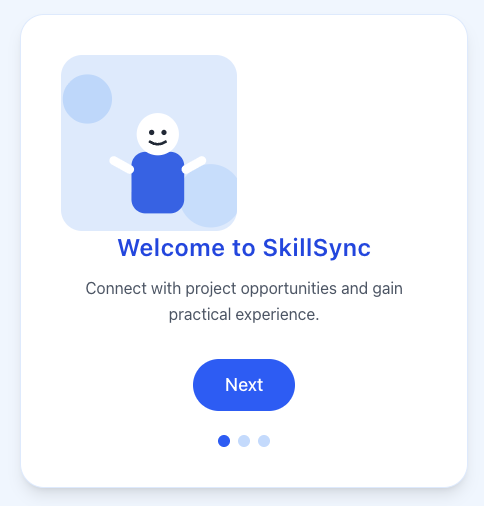
\includegraphics[width=\linewidth]{Onboarding-1.png}\\[0.3em]
      
\includegraphics[width=\linewidth]{Onboarding-2.png}
    \end{minipage}\hspace{1.5em}%
    \begin{minipage}[b]{0.42\textwidth}
      \centering
      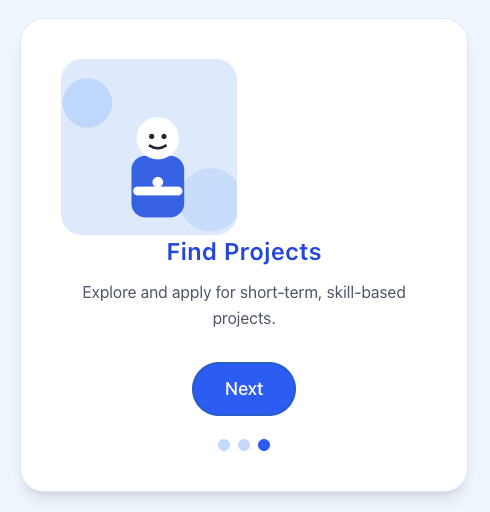
\includegraphics[width=\linewidth]{Onboarding-3.png}\\[0.3em]
      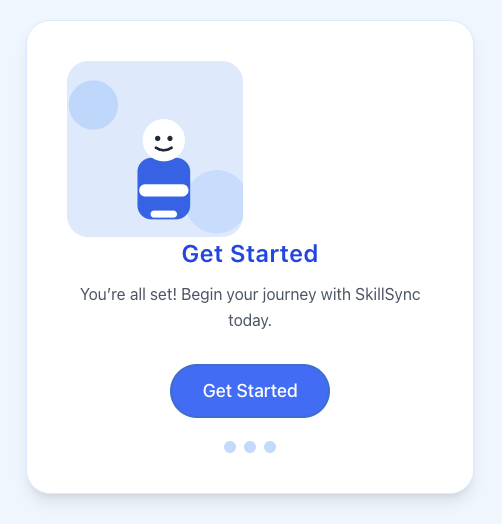
\includegraphics[width=\linewidth]{Onboarding-4.png}
    \end{minipage}}
  \caption{Guided onboarding carousel with four-step checklist.}
  \label{fig:onboarding-flow}
\end{figure}

Governance comes alive in Figure~\ref{fig:admin-panel}: the administrator dashboard gives the policy team real-time visibility into flagged content, pending disputes, and algorithm performance, with fairness metrics alongside operational stats so legitimacy does not collapse when optimising for throughput. Moderators can drill into case details, trigger templated responses, escalate to legal counsel, and rely on the audit trail for accountability reports.

\begin{figure}[H]
  \centering
  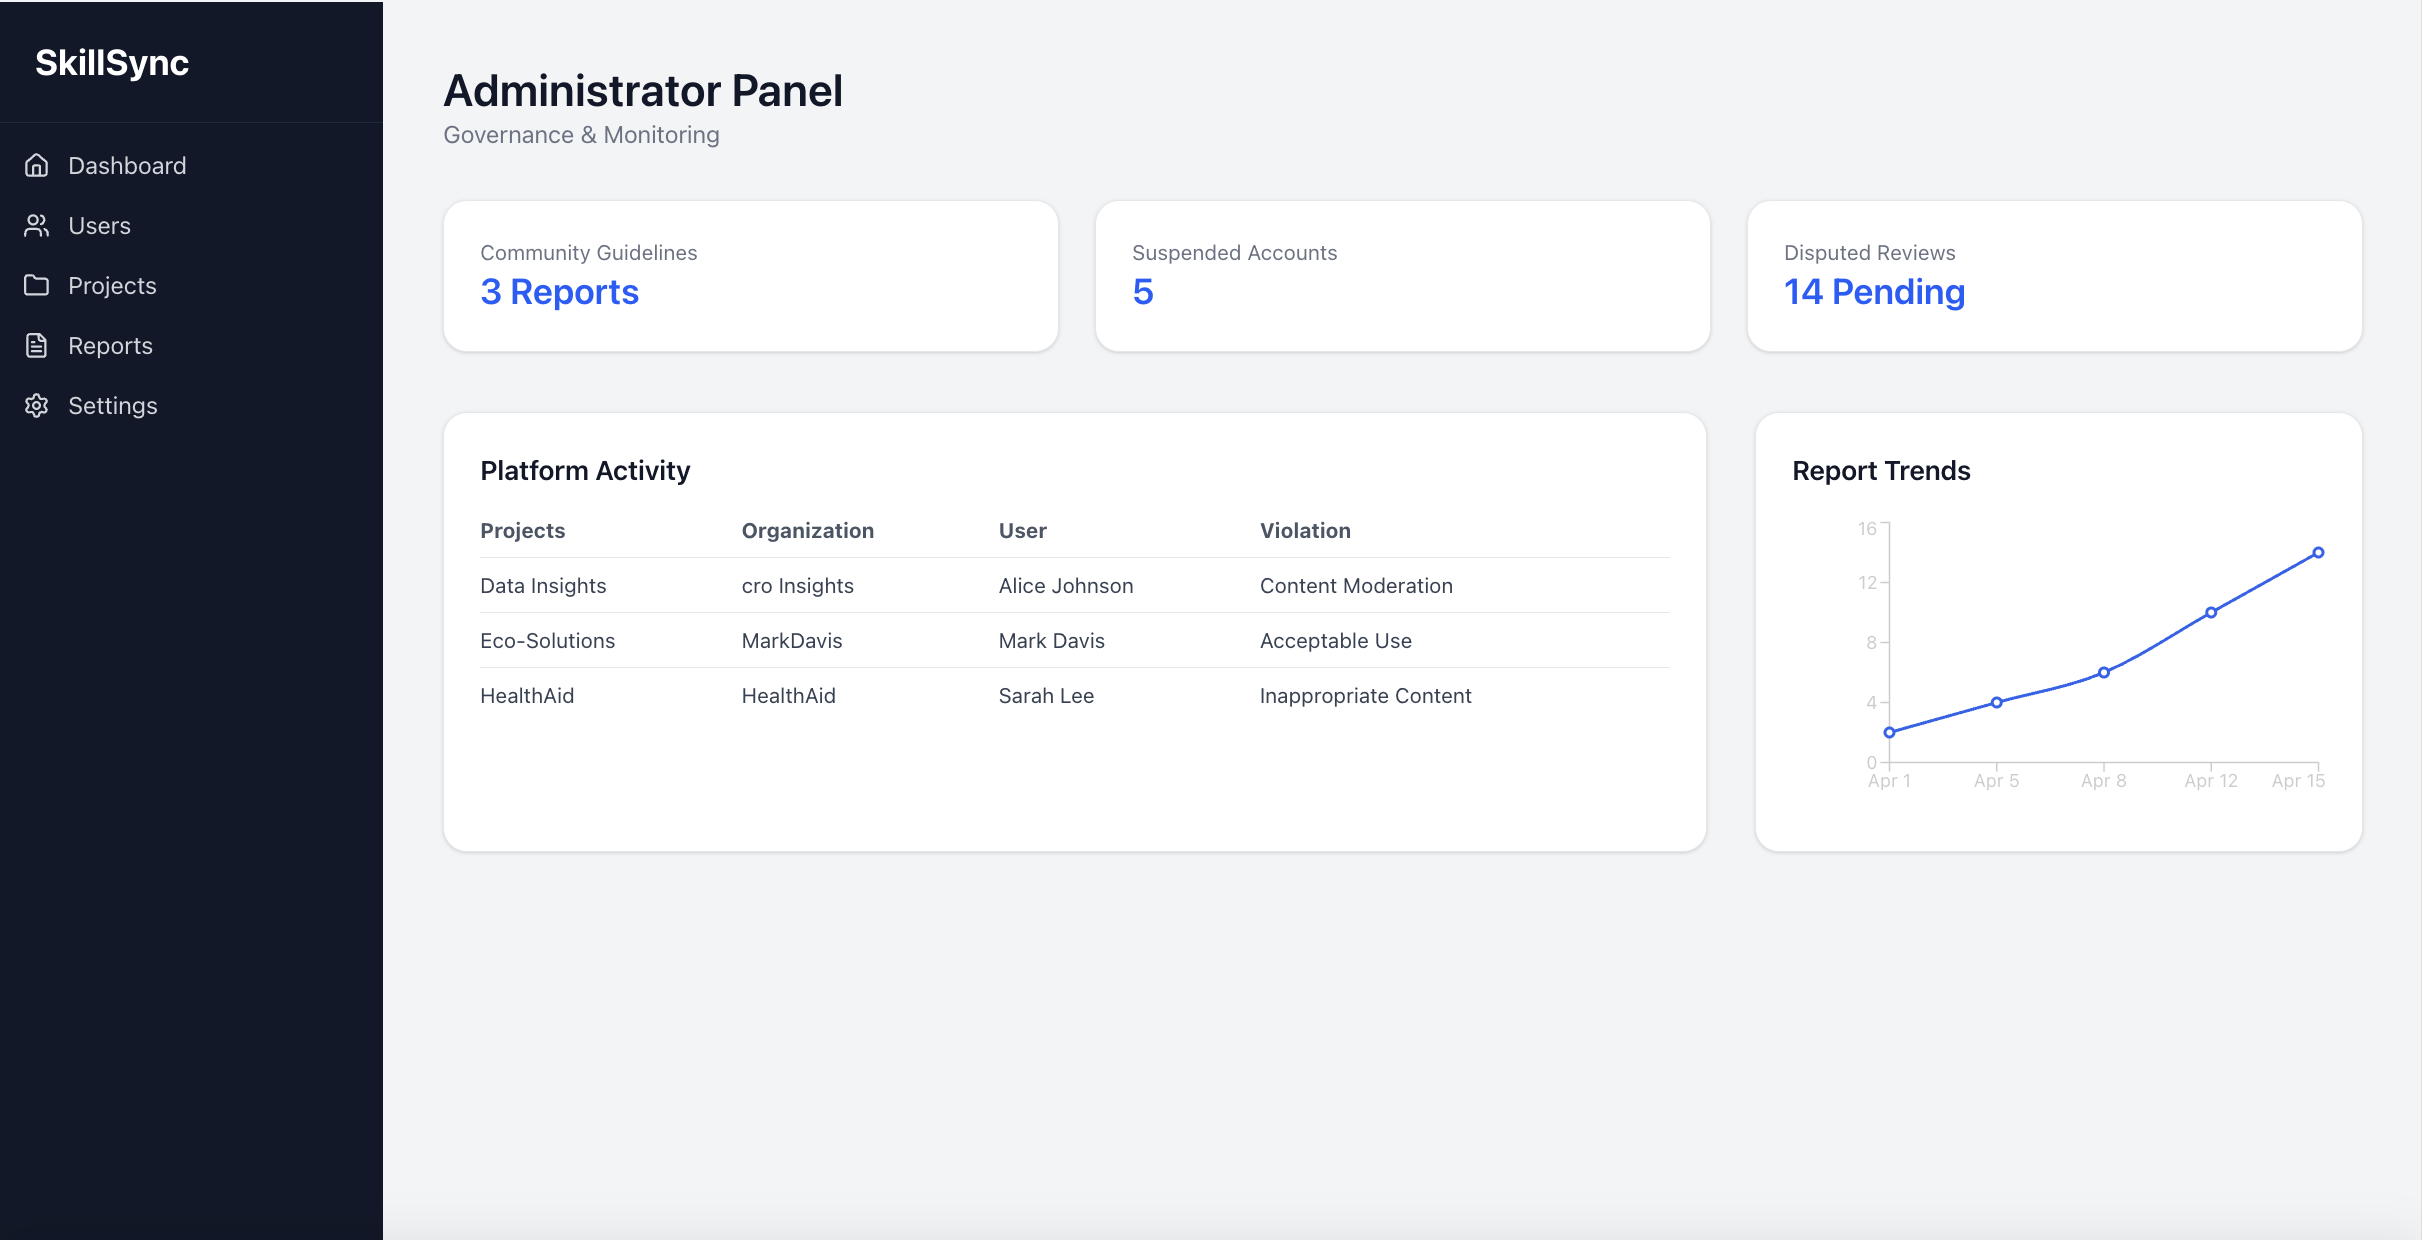
\includegraphics[width=0.85\linewidth]{Organisation-Administratorpanel.png}
  \caption{Governance control room with moderation and fairness metrics.}
  \label{fig:admin-panel}
\end{figure}

All of this hinges on communication. We script system nudges in the same human tone as onboarding, train moderators in trauma-informed responses, and host a quarterly ``town hall'' so power users can question the product team before next steps.
